\documentclass[11pt,a4paper,oneside,titlepage,openright]{book}
\usepackage{float}
\usepackage{graphicx}
\usepackage{titlesec}
\usepackage[english]{babel}
\usepackage[T1]{fontenc}
\usepackage{fancyhdr}
\usepackage{subfigure}
\pagestyle{empty}
\usepackage[utf8]{inputenc}
\usepackage{titling}
\usepackage{listings}
\usepackage{amsmath}
\usepackage{amsfonts}
\usepackage{xcolor}

\definecolor{mGreen}{rgb}{0,0.6,0}
\definecolor{mGray}{rgb}{0.5,0.5,0.5}
\definecolor{mPurple}{rgb}{0.58,0,0.82}
\definecolor{backgroundColour}{rgb}{0.95,0.95,0.92}

\lstdefinestyle{CStyle}{
    backgroundcolor=\color{backgroundColour},   
    commentstyle=\color{mGreen},
    keywordstyle=\color{magenta},
    numberstyle=\tiny\color{mGray},
    stringstyle=\color{mPurple},
    basicstyle=\footnotesize,
    breakatwhitespace=false,         
    breaklines=true,                 
    captionpos=b,                    
    keepspaces=true,                 
    numbers=left,                    
    numbersep=5pt,                  
    showspaces=false,                
    showstringspaces=false,
    showtabs=false,                  
    tabsize=2,
    language=C
}



%%ENVIRONMENT FOR ABSTRACT
\newenvironment{abstract}
{\cleardoublepage\null \begin{center}
\bfseries \abstractname \end{center}}
	{\vfill\null}
	
%%DEFINITION FOR FIRST PAGE
\makeatletter

\renewcommand{\maketitle}{%
  \let\footnotesize\small
  \let\footnoterule\relax
  \let\footnote\thanks
  \chapter*{\vspace{-3cm}\makebox[\linewidth]{\@title}}
  \begin{center}
    
\includegraphics[width=5cm]{logo}
    \vskip\dimexpr 7em-40\p@\relax%
    {\large \lineskip 0.4em%
     \textsc{Bachelor of Science in Mathematical Engineering}\\
     \vskip 0.4cm
     \Large\textsc{Bachelor degree thesis}	\\
     \vskip 1cm
     \Huge\textbf{Analysis of matrix vector product}
     \begin{tabular}[t]{c}  \@author \end{tabular}\par}%
     \vskip 3cm
    \noindent
    \parbox[t]{.5\textwidth}{\raggedright
    \large{Supervisors:}\\
    \large{Prof. Stefano Berrone}}
    \hfill
    \parbox[t]{.3\textwidth}{\raggedleft
    \large Candidate:\\
    \large{Ludovico Bessi}
    }%
    \vskip 10.7em%
    {\large \@date \par}%
  \end{center}\par
  \@thanks
  \vfill\null\setcounter{footnote}{0}
  \thispagestyle{empty}\addtocounter{page}{-1}
}
\makeatother

\begin{document} 
\title{POLITECNICO DI TORINO}
\author{}
\date{May 2019}
\maketitle

%%DEDICA
\begin{flushright}
\null\vspace{\stretch{1}}
\textit{Ai miei genitori}
\vspace{\stretch{2}}\null
\end{flushright}


%%ABSTRACT
\begin{abstract}
Comparison between different self-made implementations of the dense matrix vector product and Eigen's library implementation, using different optimizations flags on a single core.\\ After getting to the theoretical limit of performance on our machine, I addressed scalability by running the code in parallel using OpenMP. 
\end{abstract}

\tableofcontents


%%CAPITOLO 1
\chapter{Introduction}
In this first chapter I will introduce the main ideas to understand three different implementations of the code, plus the tools used to analyze them. \\
Let $\mathbf{A}$ be a $n\times n$ dense matrix and $\mathbf{v}$ be a vector of $n$ entries. We define the \textbf{kernel} as the following operation: 
$$ result[i] = result[i] + A[i,j]*vector[i]$$ 
The kernel is indeed very simple, so there is not much mathematical machinery that can be employed to speed up the calculation. \\
However, I will show how to write the code in three different ways to extract as much as performance as we can from the hardware.\\\\
When using the g++ compiler, we can set different optimization flags such as: O0, O1, O2 and O3. \\
O$0$ is the default one, and no optimization is done. From here, the higher the number the better the compiler optimizes the code.\\
The code comparison will then be done with different optimization flags and different size of matrices. Changing the dimension of the matrix shows how much difference there is in saving values in the Cache versus memory.\\\\
After that, I will address scalability by running the code in parallel using OpenMP.

\section{STREAM} 
STREAM is a simple synthetic benchmark program that measures sustainable memory bandwidth in MB/s and the corresponding computation rate for  vector kernels. \\
 Having an estimate of bandwidth is very important because it lets us calculate the performance of our code relatively to the hardware. 
By running a python script, I calculated that our bandwidth on average is: 6000 MB/s.


\section{LIKWID}
LIKWID is a set of command line tools supporting software developers, benchmarkers and application users to get the best performance on a given system.
One of the main tool is \textbf{likwid-perfctr}, that offers access to hardware performance counters and derives metrics from the raw counts. 
By running likwid-perfctr, we can profile our code. The following image is an example of an output: 

\begin{center}
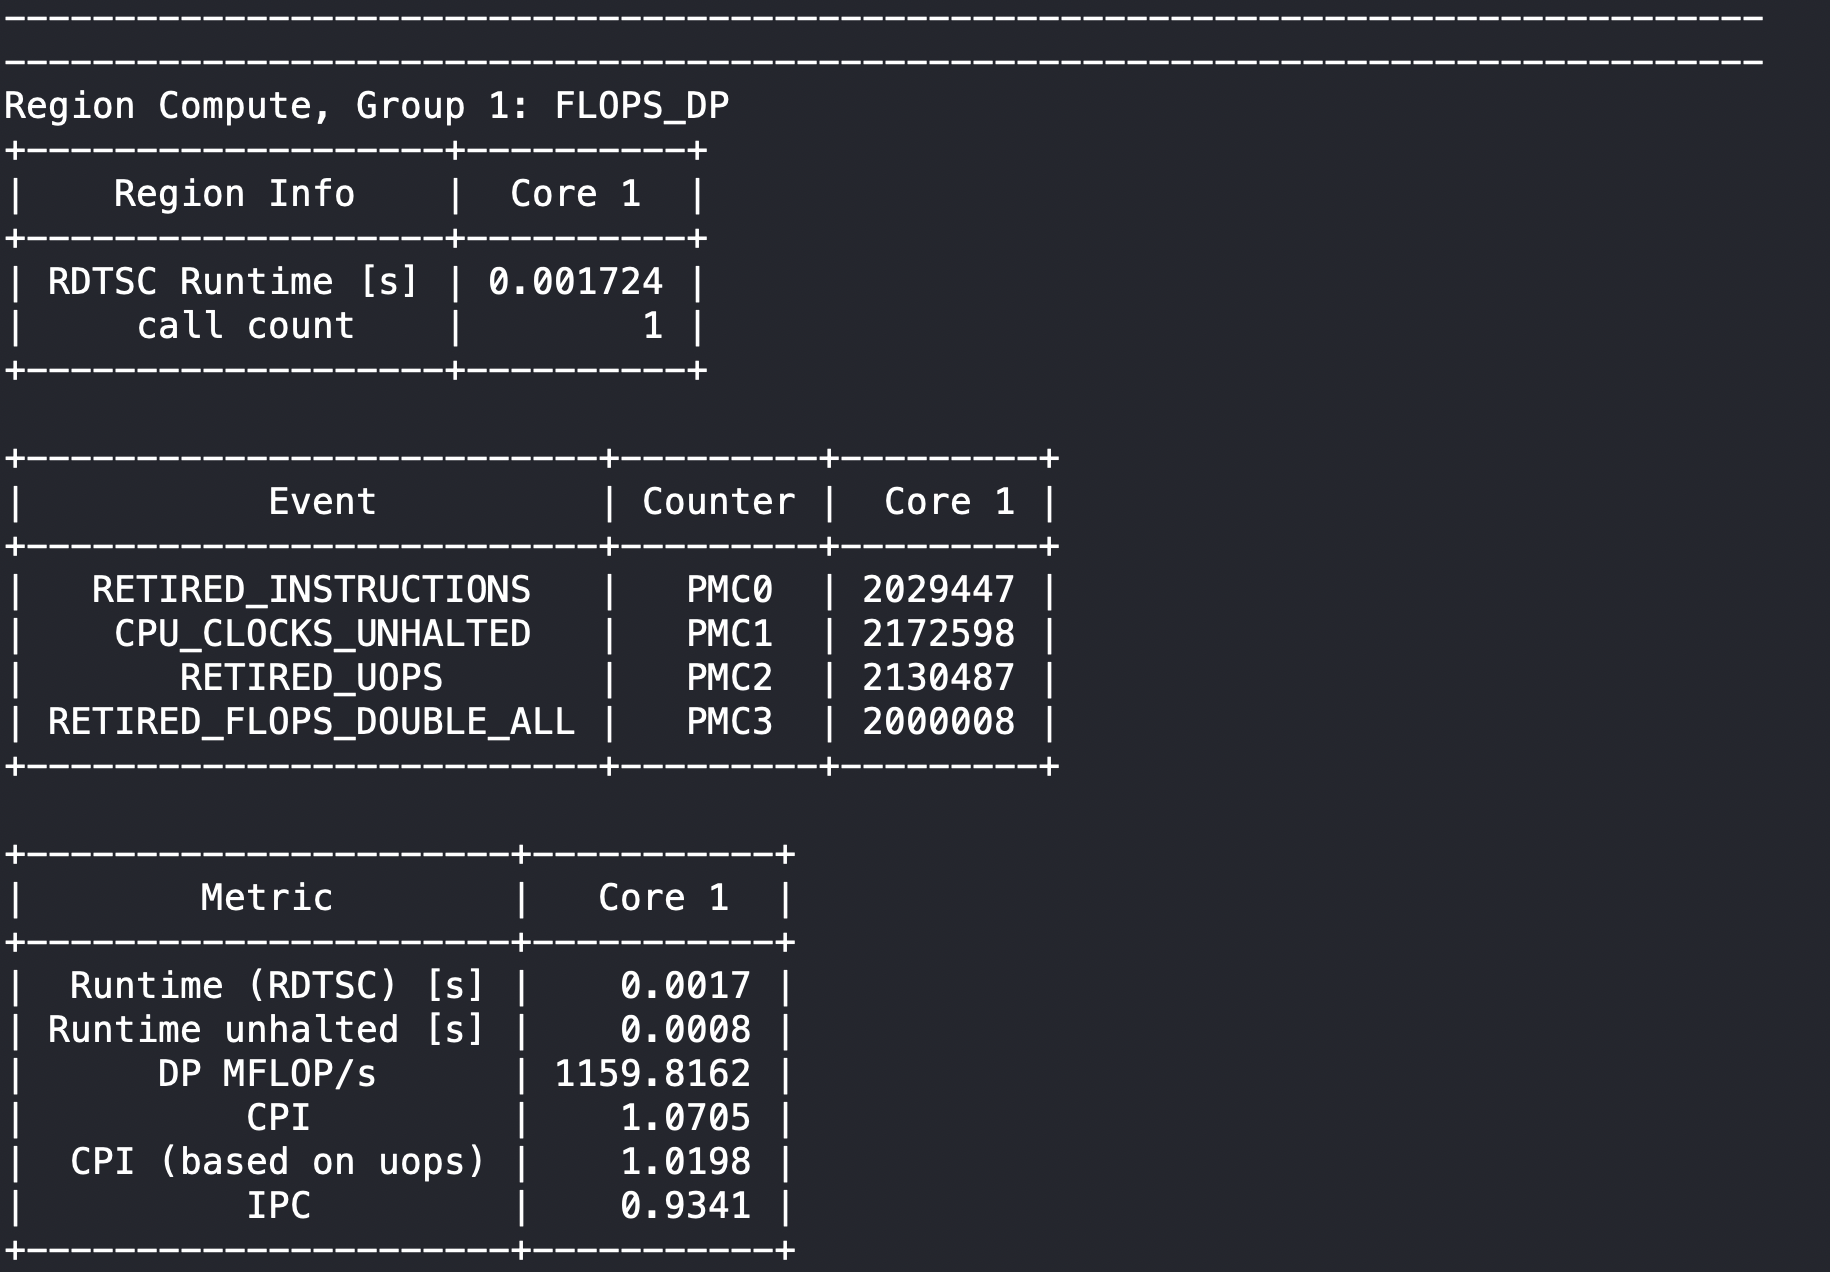
\includegraphics[width=10cm, height=8cm]{scree_lik_perf}
\end{center}

A brief explanation of all the metrics: 

\begin{itemize}
\item{\textbf{RETIRED\_INSTRUCTIONS}: instructions completely executed between two clocktick event samples.}
\item{\textbf{CPU\_CLOCKS\_UNHALTED}: number of cycles where CPU was not halted.}
\item{\textbf{RETIRED\_UOPS}: number of low-level hardware operations.}
\item{\textbf{RETIRED\_FLOPS\_DOUBLE\_ALL}: number of completely executed floating point operation per second  }
\item{\textbf{Runtime (RDTSC) [s]}: counts the number of cycles since reset. }
\item{\textbf{Runtime unhalted [s]}: counts the number of cycles since reset when CPU was not halted.}
\item{\textbf{DP MFLOP/s}:  number of double precision MFLOP/s.}
\item{\textbf{ CPI}: number of cycles per instruction retired.}
\item{\textbf{CPI (based on uops)}: Calculation of CPI based on uops.}
\item{\textbf{ IPC }: number of instructions per cycles}
\end{itemize}
Below some useful formulas that provide more insights into how these numbers are related to each other: 
\begin{itemize}
\item DP MFLOP/s = 1.0E-06*(RETIRED\_FLOPS\_DOUBLE\_ALL)/time
\item CPI = CPU\_CLOCKS\_UNHALTED/RETIRED\_INSTRUCTIONS
\item CPI (based on uops) = CPU\_CLOCKS\_UNHALTED/RETIRED\_UOPS
\item IPC = RETIRED\_INSTRUCTIONS/CPU\_CLOCKS\_UNHALTED
\end{itemize}
To understand and use the performance properties of the hardware, it is important to know the machine's topology: \textbf{likwid-topology} gives us information about: 
\begin{itemize}
\item \textbf{Thread topology}: how threads are concurrently executed and split in subprocesses. 
\item \textbf{Cache topology}: how processors share the cache hierarchy.
\item \textbf{Cache properties}: detailed information about all cache levels.
\end{itemize}
Below an example of the output with information about HW and thread topology:\\
\begin{center}
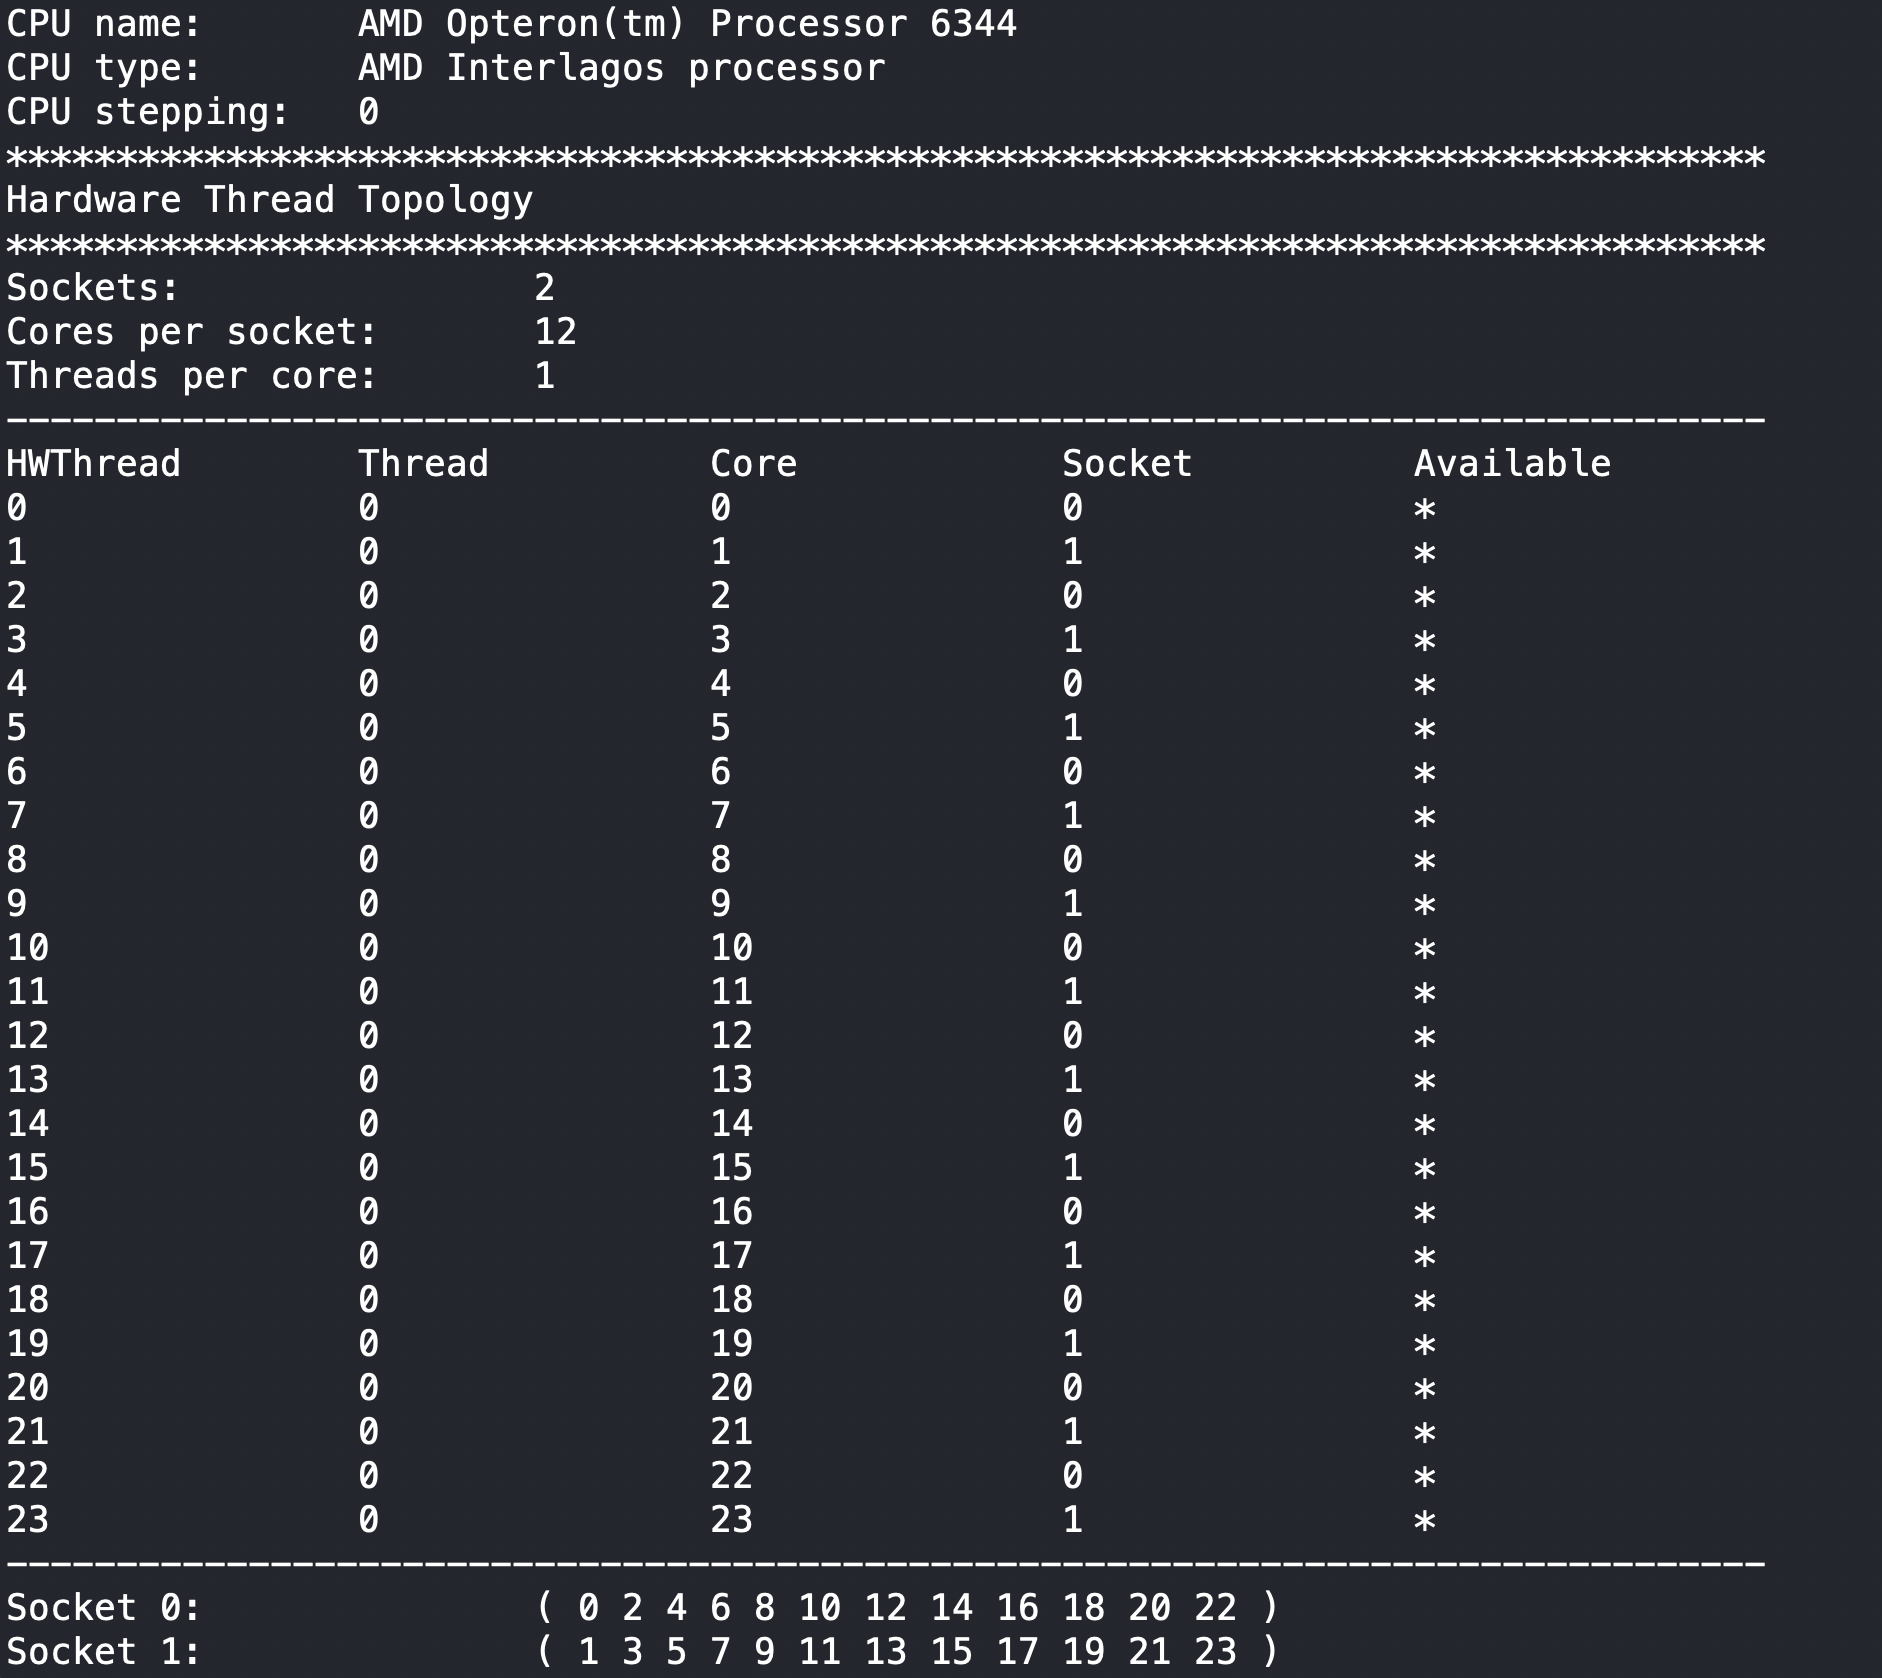
\includegraphics[width=10cm, height=8cm]{topology_1}
\end{center}
Another picture with information on cache levels:\\
\begin{center}
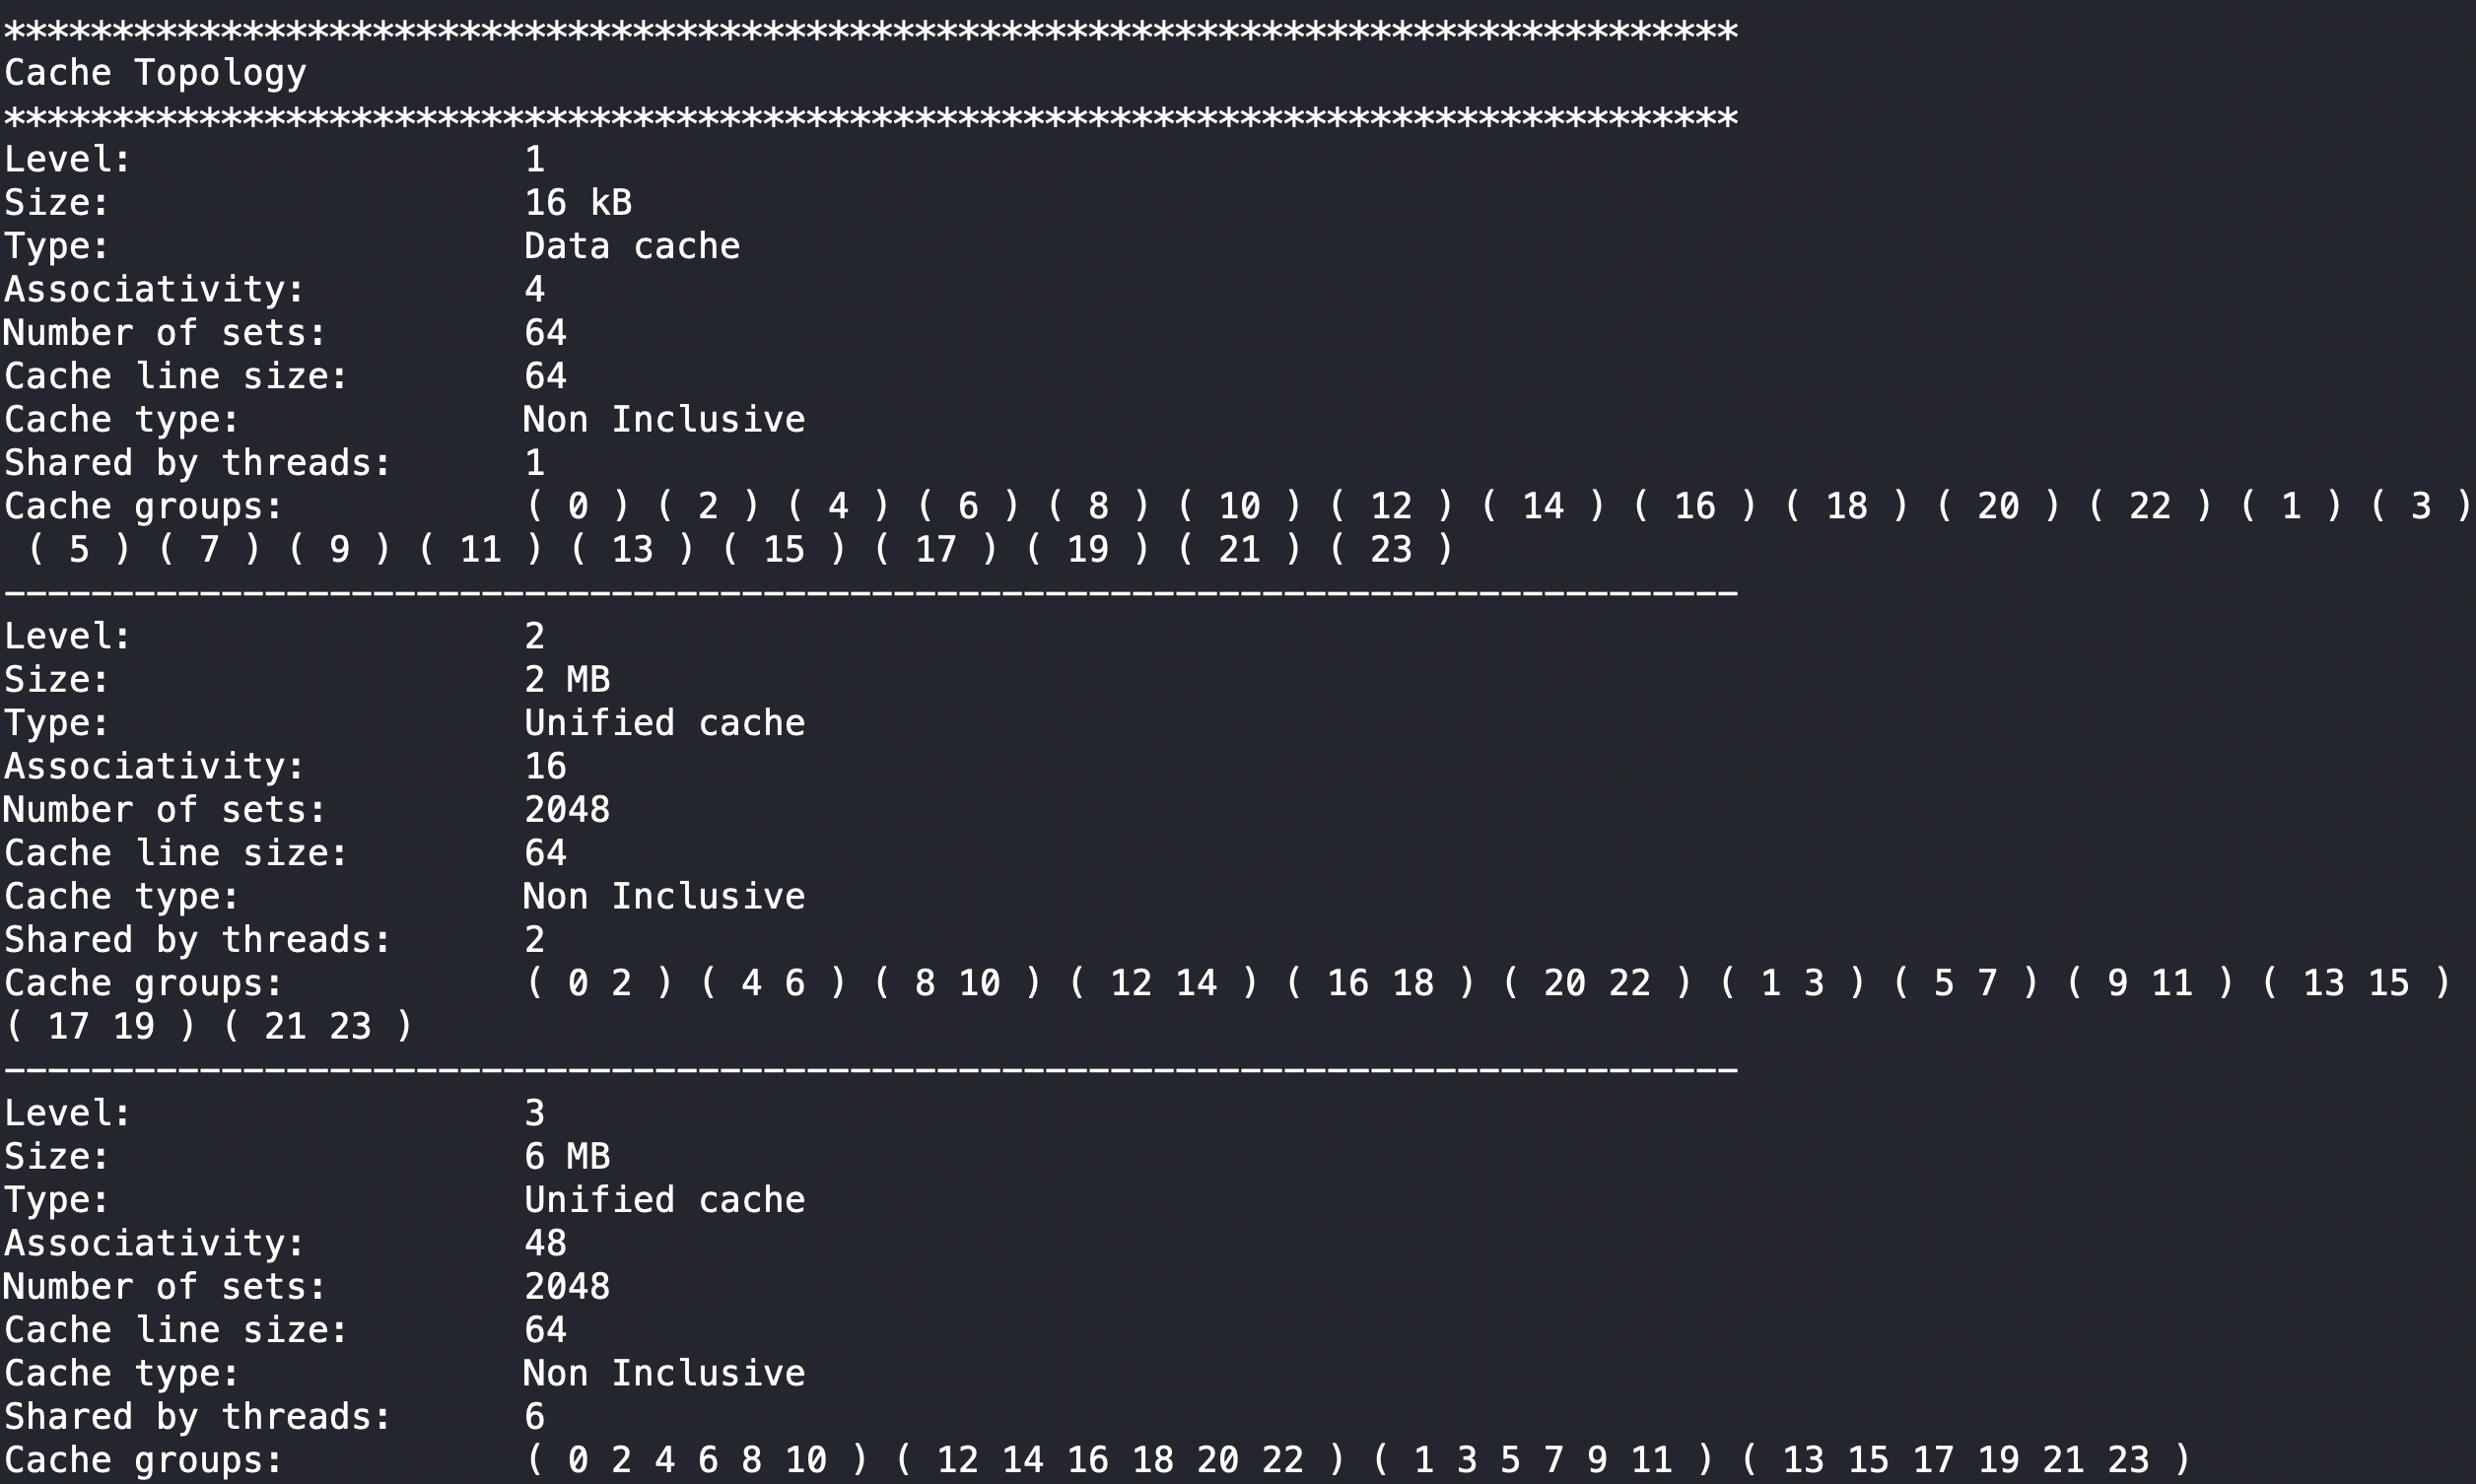
\includegraphics[width=10cm, height=8cm]{topology_2}
\end{center}
Lastly, likwid let us change the maximum and minimum frequency of our CPU. To have the least amount of oscillations when running our code, we set both at 2.6GHz, which is the maximum frequency allowed by our machine.

\section{Hardware specifications}
The Interlagos 12-core (for each socket) Opteron processor by AMD's. We  The cores are paired into "modules" which share a significant proportion of resources. The figure below gives an overview of which resources are shared between the two cores of a module. More information can be found here: \cite{interlagos}

\begin{center}
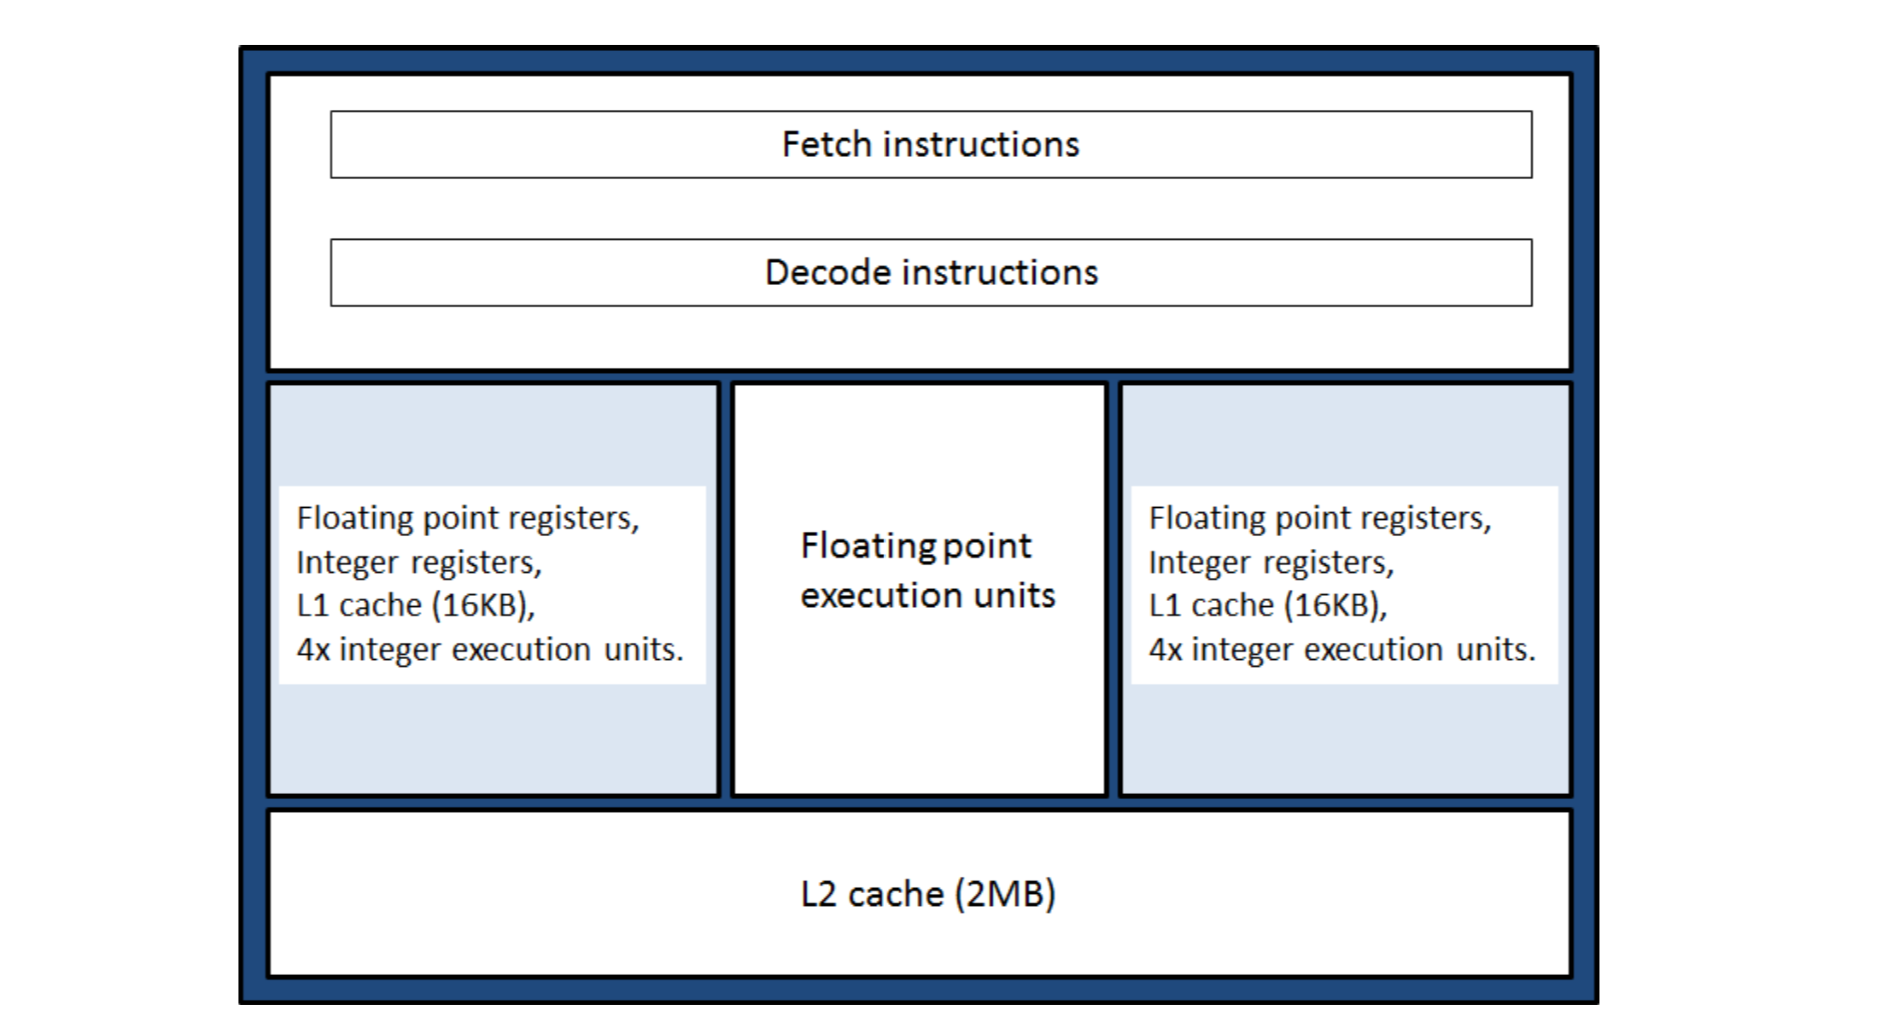
\includegraphics[width=10cm, height=8cm]{interlagos}
\end{center}

\section{Eigen}
Our main goal is to see how our code measures against Eigen's. 
Eigen is a library written in C++ which provides algorithms for fast matrix algebra, such as: dense and sparse product of matrix and vectors, matrix decomposition, space transformations. \\This library is widely used by many projects and is the result of the work of experts starting at least from 2009. Given this premises, it seems very difficult to get close to their performance. However, even matching it will be a great accomplishment and would show that there is still work to be done to improve it. 

\section{Roof-line model}
The Roofline model is a performance model used to provide estimates of a given computer kernel. 
It can be visualized by plotting floating point performance as a function of arithmetic intensity. \\\\
This model is used to determine the two main bottlenecks: bandwidth and algorithm's perfomance. It works under the assumption that data is already saved in cache and there  is no latency. It depends on empirical measurements, so it is inherently subject to error. 
It plots the performance of the code as dependent variable of computational intensity, below I will explain how to calculate such values using the tool described at the beginning of the chapter. 
\\
The peak performance can be calculated using the following formula, where $n$ is the number of cores, $F$ is the number of floating point instructions for cycle, $v$ is the clock speed and $S$ is the SIMDY feature, for now we are not concerned about this last term. 
$$ P_{peak} = n * F * S * v $$ 

We can also define the maximum performance reached by our machine with the following formula, where $f_{max}$ is the maximum frequency of the CPU of our machine, $\frac{n_{operations}}{n_{cycles}}$ is the number of operations per cycle. 
$$P_{max} = f_{max} * \frac{n_{operations}}{n_{cycles}}$$ 

In our case, the result is then just 2.6$\frac{Gflops}{s}$.
However, this is just the theoretical limit: our performance P actually is: 

$$ P = min(P_{max}, \text{Bandwidth * computational intensity}) $$
In this formula, computational intensity is s a measure of floating-point operations (FLOPs) performed by a given code (or code section) relative to the amount of memory accesses (Bytes) that are required to support those operations. \\
We shall see how it is indeed the deciding factor when evaluating different algorithms, because in this framework we ideally want to build an an algorithm such as that the value $\textbf{Bandwidth * computational intensity}$ reaches $P_{max}$.\\\\
With this idea in mind, I developed three different implementations of the dense matrix vector product:

\begin{itemize}
\item \textbf{Naive implementation}: the classic implementation, still useful to benchmark against to check progress. 
\item \textbf{Temporary variable}: using a temporary variable saved in cache to  lessen the number of fetches from memory. 
\item \textbf{Loop unrolling}: splitting up the loop manually to exploit pipe levels, that means keeping the pipe occupied avoiding  downtime. Moreover, we manage to get more temporary variables in cache.
\end{itemize}
After the last implementation, we adressed scalability. That is, we looked at how our kernel worked in parallel using OpenMP.




%%CAPITOLO 2
\chapter{Naive implementation}

The naive implementation is just that, the simplest code one can develop to solve this problem, below the .C file:
\lstinputlisting[style=CStyle]{naive_without_tmp.c}
The computational intensity in this case is $\frac{2}{32}\frac{Flops}{Bytes}$. 
\\Before blindly applying the formulas seen in chapter one, there are some key insights to understand. Until we get to the final implementation, we are not exploiting pipelines of sum and product. In short, this means that we are not allowing the processor to execute these basic operations in parallel. It follows that $P_{max}$ is limited by a factor of $8$, because the size of the pipe for sum and of product are 4 each.
We then have that $P_{max}= \frac{2.6}{8} \frac{Gflops}{s} $, and this is a major bottleneck of our program, because $\textbf{Bandwitdht} * \textbf{computational intensity} = 6*\frac{1}{16} = 0.375 \frac{Gflops}{s} $. We will tackle the bottleneck in chapter 4.\\
Using likwid-topology, we find the following sizes for the cache: 
\begin{itemize}
\item L1: 16 kB
\item L2: 2 MB
\item L3: 6 MB
\end{itemize}
We are going to focus our attention on the L1 and L2 cache levels, which are the fastest. In short: if the elements we are working with are saved there, we can access them faster than usual.  For dense matrices, L2 is actually faster than L1. I am going to repeat the same analysis with three different matrices of size respectively $n_1 = 40$, $n_2 = 400$, $n_3 = 1000$.\\
The first matrix can be saved in L1, the second one in L2 and the third one is saved in memory.  


%%CAPITOLO 3
\chapter{Temporary variable}

We can improve the code described in chapter two, introducing a temporary variable in the following way: 
\lstinputlisting[style=CStyle]{naive_with_tmp.c}
At first glance, It may seem we are just wasting precious cache space with another double variable but it turns out this change doubles the computational intensity with respect to the first algorithm. \\
The key take away is that our kernel does not change even with the addition of the $\textit{tmp}$ variable: this time we can skip the fetching and loading of this variable, because when entering the second for loop it is already in the cache. This means that the computational intensity becomes $\frac{2}{16}\frac{Flops}{Bytes}$. 
However, we still have not solved the pipeline's problem described in the previous chapter. \\
This means that even though we doubled the computational intensity our bottleneck is still $P_{max}$ due to the coefficient $\frac{1}{8}$.  
Nevertheless, by compiling the code we still manage to improve, as seen in chapter 5.


%CAPITOLO 4 
\chapter{Loop unrolling}
With this code, I finally manage to exploit the sum and product pipelines, thus reaching $P_{max}$ = 2.6 GHz, then the bottleneck must be in the other term, which depends on the computational intensity of the algorithm. 
The code can be found below: 
\lstinputlisting[style=CStyle]{loop_unrolling.c}
The pipeline for the sum and multiplication is constantly filled with the trick of splitting the loop 4 by 4. It can be seen as a generalization of the code with the temporary variable. \\\\
This time, the computational intensity is $\frac{32}{160}\frac{Flops}{Bytes}$. In the numerator we have 32 operations. In the denominator we get 160 by seeing that we fetch and load $(16+4)$ double elements, thus getting 160 bytes. 
Then the operational intensity is $\frac{1}{5}\frac{Flops}{Bytes}$, multiplied by the Bandwidth we get 1.2 $\frac{Gflops}{s}$. 

\section{Analysis of Assembly code} 
It is also useful to take a look at how the compiler arranges instructions at a lower level. Below, a side by side comparison of a snippet of C code and Assembly code: 
\begin{center}
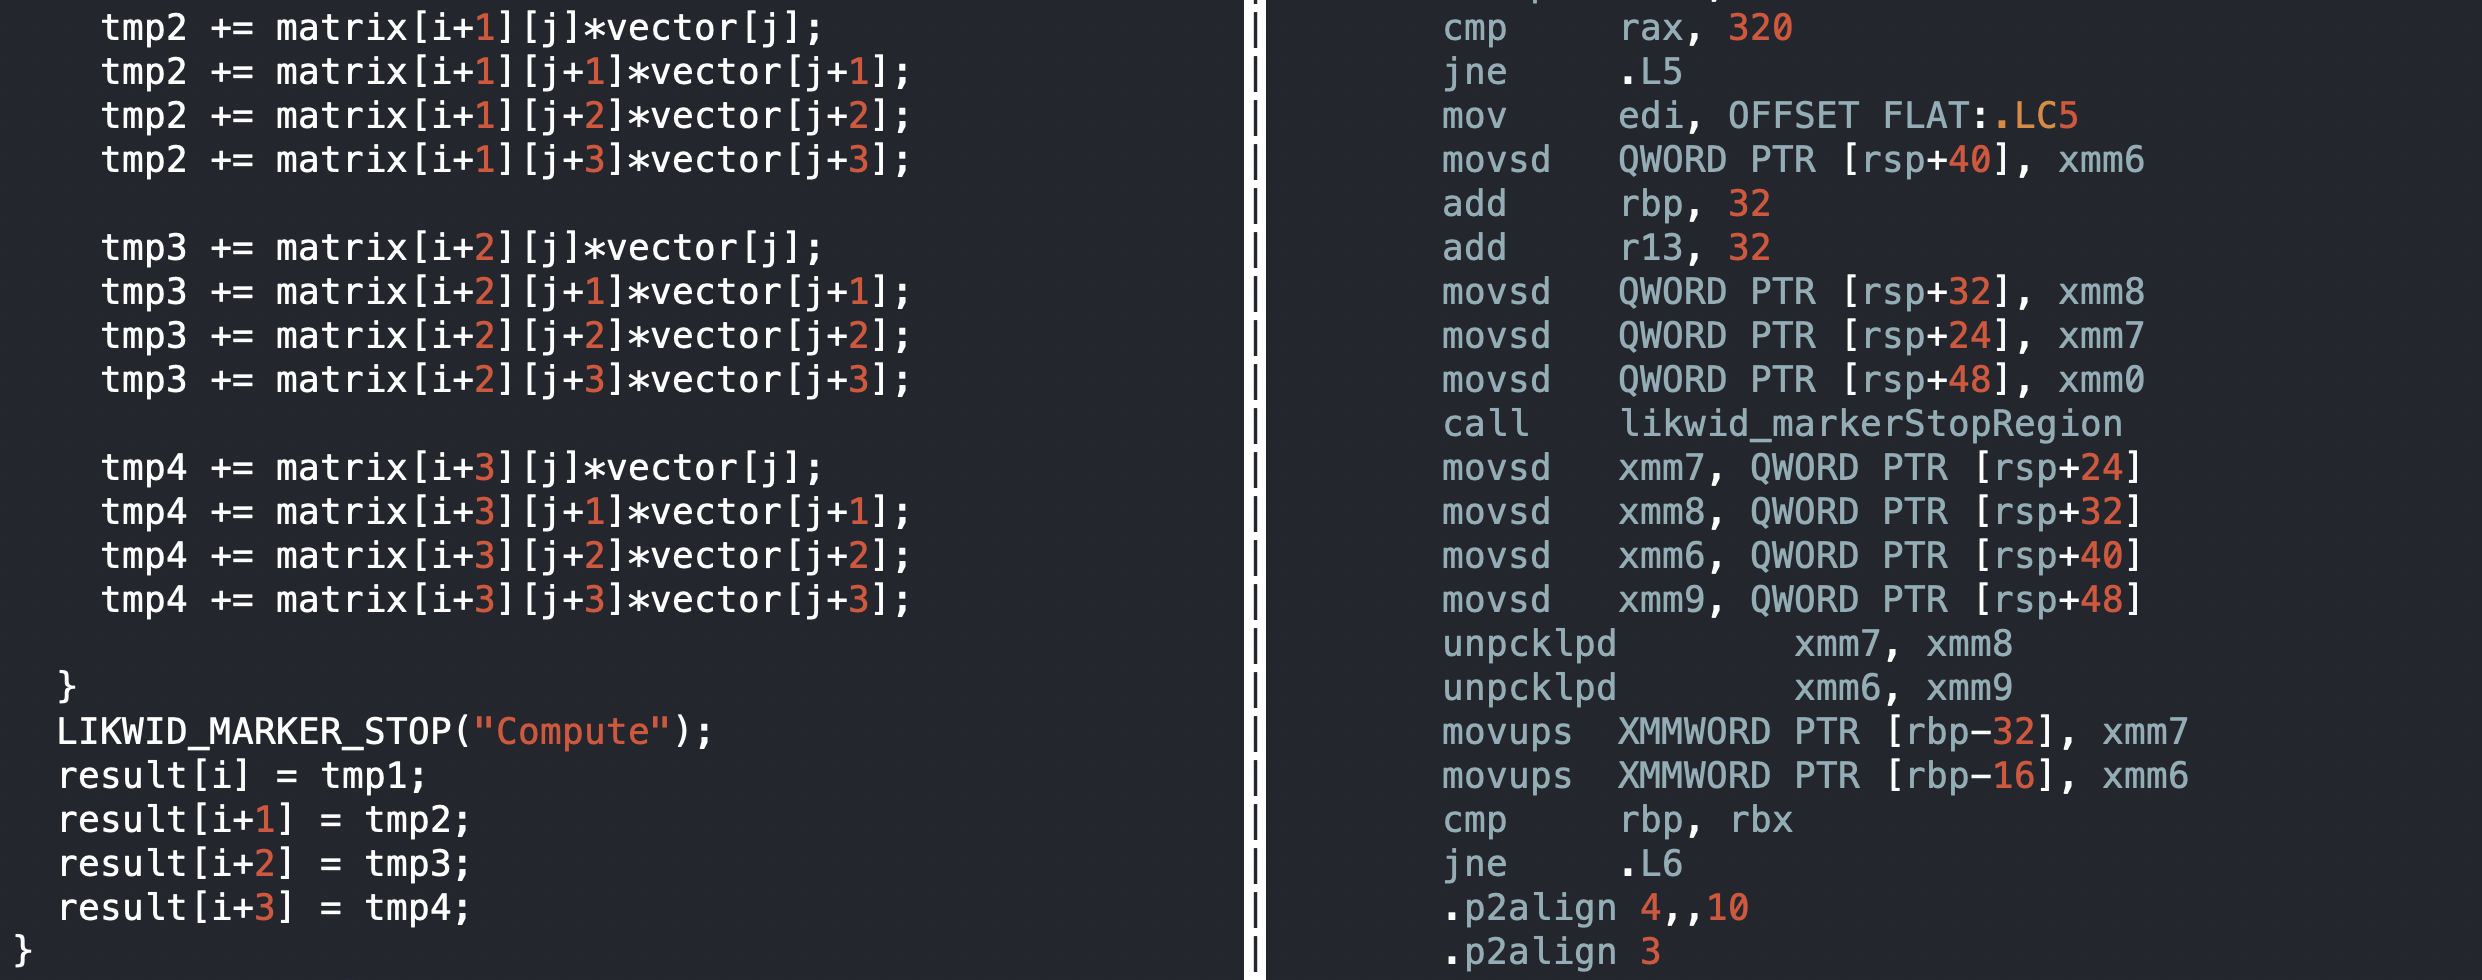
\includegraphics[width=14cm, height=7cm]{assembly_screen}
\end{center}
The easiest piece to recognize is the call to the function \textit{likwid marker stop}. In our source code, after that call we assign 4 double values to specific entries of the result vector. We can see in the Assembly code that we have 4 \textbf{movsd} calls, which moves a scalar double-precision floating-point value to another location.\\ A few lines after that, we can see the word \textbf{cmp} which stands for compare, this is checking the condition on the for loop, if it satisfied it jumps at the beginning again with the call \textbf{jne}.

%CAPITOLO 5 
\chapter{Eigen implementation and comparison}

Let's now see how the the Eigen library is doing on the same hardware. 
Below four tables that represent the data gathered from the simulation, every number is expressed in MFlops/s.

\begin{center}
 \begin{tabular}{|c c c c c |} 
 \hline
 O0 & naive   & with\_tmp & loop unrolling & eigen \\ [0.5ex] 
 \hline
 n = 40 & 195   & 204       & 313          & 59    \\ 
 \hline
 n = 400 & 328   & 332       & 453                 & 70       \\
 \hline
 n = 1000 & 327  & 328    &  445            & 94   \\
 \hline
\end{tabular}
\end{center}


\begin{center}
 \begin{tabular}{|c c c c c |} 
 \hline
 O1 & naive & with\_tmp & loop unrolling & eigen \\ [0.5ex] 
 \hline
 n = 40 & 302 &  255 & 882  & 464\\ 
 \hline
 n = 400 & 948 & 345 & 2346 & 2339\\
 \hline
 n = 1000 & 740 & 344 & 1544 & 1922\\
 \hline
\end{tabular}
\end{center}

\begin{center}
 \begin{tabular}{|c c c c c |} 
 \hline
 O2 & naive & with\_tmp & loop unrolling & eigen \\ [0.5ex] 
 \hline
 n = 40 & 313 & 315 & 926  & 455\\ 
 \hline
 n = 400 & 941 & 937 & 3046 & 2297\\
 \hline
 n = 1000 & 720 & 704 & 1523 & 1958\\
 \hline
\end{tabular}
\end{center}

\begin{center}
 \begin{tabular}{|c c c c c |} 
 \hline
 O3 & naive & with\_tmp & loop unrolling & eigen \\ [0.5ex] 
 \hline
 n = 40 & 315 & 321 & 915  & 383\\ 
 \hline
 n = 400 & 936 & 961 & 2935 & 3429\\
 \hline
 n = 1000 & 761 & 766 & 1538 & 2024\\
 \hline
\end{tabular}
\end{center}
Let's see what are the main takeaways from the data.\\
For $n = 40$, Eigen struggles against our best implementation for every flag by a pretty significant margin. \\
The code performs better with $n = 400$ than with $n = 40$, which seems strange at first because L1 cache should be faster than L2. However it seems to be a known issue that for dense matrix product the gcc compiler does not to exploit all the performance. I am going to analyze this issue in greater detail in the next section.\\\\
Unsurprisingly, the code runs faster with $n = 400$ than with $n = 1000$. One reason is the fact that the elements of the latter are saved in memory. 
We see that Eigen performs the best when the compiler setting are turned to the maximum. Otherwise, loop unrolling performs very well.\\\\ 
It is very interesting to see how much performance we gained from the first implementation to the third one. It is summarized in the graph below where the data is taken from the -O2 compilation.

\begin{center}
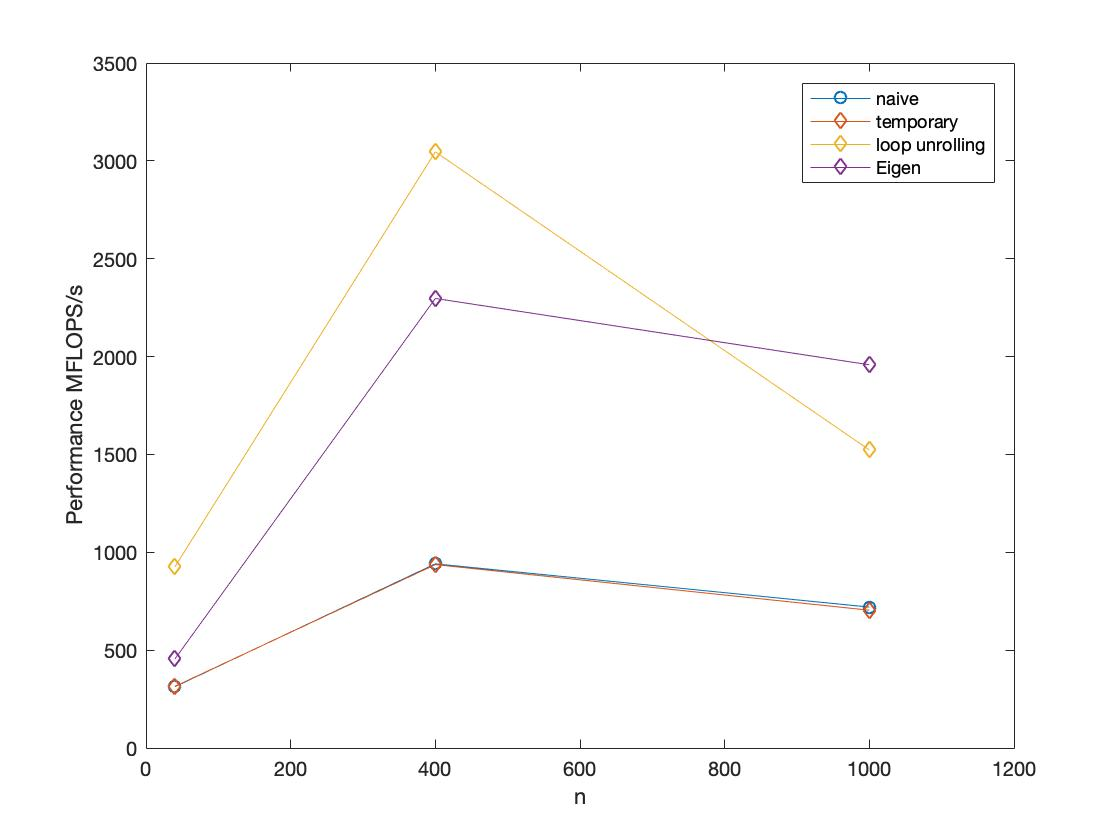
\includegraphics[width=10cm, height=8cm]{plotcolor}
\end{center}
To really understand what is going on at the lowest level, we can take a look at the assembly code for eigen loop unrolling.\\\\
A brief analysis on the model used:\\
Our roofline graph is the following: 
\begin{center}
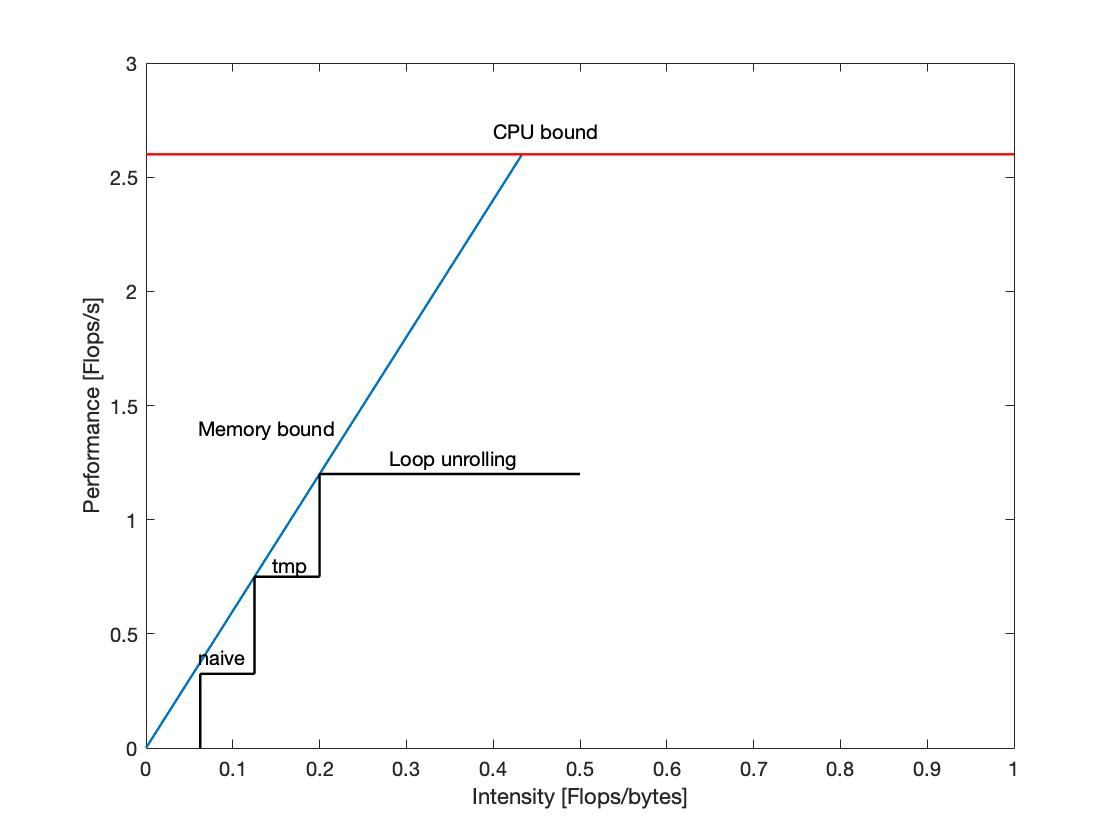
\includegraphics[width=10cm, height=8cm]{fig_ok}
\end{center}
Based on the model we chose, our performance should not have surpassed 1200$\frac{MFlops}{s}$. However our code reaches on average a maximum performance of 2935 $\frac{MFlops}{s}$ and Eigen a staggering 3429 $\frac{MFlops}{s}$. 
However, the roof line model struggles to represent the gains made by exploiting cache levels. If we used the roofline cache aware model, seen in \cite{roofmdelcache} the model would have been closer to reality. 
Moreover, even by setting the frequency of the CPU to a constant value, it still fluctuates a bit because of the \textit{Turbo Boost} feature of our hardware. 
Basically, the operating system may decide to up the frequency of the CPU for a short time if it is deemed useful for the task at hand.

\subsection{In-depth analysis of $n = 40$ performance}

With $ n = 40$, we have the big advantage of saving everything in the L1 cache. However, it is hard to use our metrics to appreciate the gain because we have very little execution time, in the order of $10^{-5}$. Moreover, LIKWID performs heavy approximation in its calculations. \\
With $n= 400$, we get a run time of the order of $10^{-4}$. The idea is to artificially increase the flops in the $n=40$ case to achieve the same order of magnitude and be able to compare the two. We achieve the result by adding another for loop that does nothing, and enlarge the section of code that LIKWID analyzes. 
By doing this, we get a better result for $n = 40$, even though $n = 400$ is still performing better. 


%CAPITOLO 6
\chapter{Parallel computations using OpenMP}

\textbf{Open Multi-Processing} is an application programming interface that supports multi-platform shared memory multiprocessing. It is used for parallelism within a multi-core node.\\ It is based on threads, which are processes that can share memory. \\They communicate with each other via reading and writing shared data. 
Each thread proceeds through program instructions independently of other threads, that means it is important to ensure that actions on shared variables occur in the correct order.\\\\
In many applications, loops are the main source of parallelism. If the iterations can be done in any order, it is possible to share the iterations between threads, for instance: thread \#1 does the even iterations and thread \#2 does the odd. After the loop is done, we can merge together the result of the two loops. In theory, we managed to do the same task in half the time.\\\\
I will run the naive code with $n = 50000$, $O3$ flag, with number of threads 1,2,4,6 to appreciate the difference in run time. Moreover, I will also analyze how LIKWID counts the run time using a double variable inside the code.\\\\ 

TO DO TWO GRAPHS for times 

%CAPITOLO 7 CONCLUSIONI AND FUTURE DIRECTIONS?
\chapter{Future directions}
SIMDY 
%%BIBLIOGRAPHY
\begin{thebibliography}{1}

\bibitem{likwid} 
Jan Treibig, Georg Hager, Gerhard Wellein, \textit{LIKWID: A lightweight performance-oriented tool suite for x86 multicore environments.}
 
\bibitem{openmp}
Mark bull, \textit{A Short Introduction to OpenMP.}

\bibitem{eigen}
Ga\"{e}l Guennebaud, Beno\^{i}t Jacob, \textit{Eigen v3}

\bibitem{roofmodel}
Samuel Williams, Andrew Waterman, David Patterson, \textit{An insightful visual performance model for floating point programs and multicore architectures.}

\bibitem{roofmdelcache}
Aleksandar Illic, Leonel Sousa, Frederico Pratas, \textit{Cache aware roofline model: Upgrading the loft.}

\bibitem{loop_unrolling}
Hewlett-Packard Development Company, \textit{Loop unroll and jam.}

\bibitem{interlagos}
Numerical Algorithms Group Ltd, \textit{How to make best use of the AMD Interlagos processor.}
\end{thebibliography}
 
\end{document}




